%%%%%%%%%%%%%%%%%%%%%%%%%%%%%%%%%%%%%%%%%%%%%%%%%%%%%%%%%%%%%%%%%%%%%%%%%%%%%%%
%
%               LaTeX-Template for theses at the PST group.
%
% Authors:
%       Matthias Hölzl/Moritz Hammer, 2006
%       Annabelle Klarl 2011
%%%%%%%%%%%%%%%%%%%%%%%%%%%%%%%%%%%%%%%%%%%%%%%%%%%%%%%%%%%%%%%%%%%%%%%%%%%%%%%

\documentclass{thesisPST}
% macros for theses at the PST group
% 
% Matthias Hölzl, 2006
% Annabelle Klarl, 2011

\usepackage{listings} % source code printer package

% for code snippets -> see also http://www.ctan.org/tex-archive/macros/latex/contrib/listings/listings.pdf
\lstnewenvironment{pseudocode}[1][]
{\lstset{
	language=Java,
	tabsize=3,
	mathescape=true,	
	frame=single,
	framexleftmargin=5mm,
	xleftmargin=0cm,
	%aboveskip=,
	%belowskip=,
	%backgroundcolor=\color{yellow},
	escapeinside='',
	showstringspaces=false,
	captionpos=b,
	numbers=left,
	numberstyle=\tiny,
	stepnumber=1,
	numbersep=5pt,
	%firstnumber=100
	basicstyle=\footnotesize\ttfamily,
	keywordstyle=\bf,
	morekeywords={},
	deletekeywords={},
	identifierstyle=,
	commentstyle=\color{grey},
	escapechar=§
	}
}{}

\begin{document}

%%%%%%%%%%%%%%%%%%%%%%%%%%%%%%%%%%%%%
%% Change according to your thesis %%
%%%%%%%%%%%%%%%%%%%%%%%%%%%%%%%%%%%%%
% change according to your thesis (german or english!)
\thesisType{Bachelorarbeit} 
\thesisAuthor{Jonas Kemper}
\thesisProgram{Medieninformatik Bachelor}

\thesisTitle{Minecraft in MicroPsi}

% Do not delete this command!
% If you do not have a a subtitle, leave it empty!
\subtitle{Eine populäre Videospielwelt als Simulationsumgebung für eine kognitive kuenstliche Intelligenz}

\referee{Prof.~Dr.~Martin Wirsing}
\supervisor{Joscha Bach~PhD, Annabelle Klarl}

\handInDate{19. September 2013}

%\selectlanguage{ngerman}
\selectlanguage{english}

% use this command to define syllable division for special words (e.g. class names)
\hyphenation{Be-ant-wortung}

%%%%%%%%%%%%%%%%%%%%%%%%%%%%%%%%%%%%%
%%%%%%%%%%%%%%%%%%%%%%%%%%%%%%%%%%%%%

\frontmatter % for Roman numbering 
\maketitlepage
\cleardoublepage
\selbststaendigkeitserklaerung
\cleardoublepage
\pagestyle{headings}

%%%%%%%%%%%%%%%%%%%%%%%%%%%%%%%%%%%%%
%% Change according to your thesis %%
%%%%%%%%%%%%%%%%%%%%%%%%%%%%%%%%%%%%%

\chapter*{\centering \begin{normalsize}Zusammenfassung\end{normalsize}}
\begin{quote}


Simulationsumgebungen spielen für das Testen und Erforschen von neuen Ansätzen für künstliche Intelligenz eine entscheidende Rolle. Da sich Computerprogramme nur mit erhöhtem technischen und finanziellen Aufwand in die physische Welt implementieren lassen, können simulierte Umgebungen schnellere, günstigere und reproduzierbarere Ergebnisse liefern. Genauso wie Innovationen aus dem Bereich der KI neue Impulse setzen, können auch neue Ansätze für Simulationsumgebungen zu neuen Erkenntnissen führen.

Das populäre Videospiel Minecraft bietet sich durch die kompositionale Semantik der Spielwelten besonders als Grundlage für eine Simulationsumgebung an, da das Agentensystem durch das Erforschen seiner Umwelt, Wissen über die Spielwelt aufbauen und sich ähnelnde Strukturen wiedererkennen kann. Objekte der Spielwelt sind in Minecraft keine bloßen Hindernisse, sondern werden mit variablen Eigenschaften prozedural generiert. Durch die Komposition dieser Objekte entstehen Umgebungen, die einer realen Umgebung in dieser Hinsicht eher gleichen, als andere virtuelle Welten. Da Minecraft einen umfangreichen Mehrspielermodus beinhaltet, lässt es sich zudem für Multiagenten-Umgebungen und so für Simulationen mit kollaborativen Agenten verwenden. Darüber hinaus sind Minecraft-Lizenzen günstig zu erwerben, erhältlich für viele Plattformen und es gibt eine äußerst große und aktive Community für selbsterstellte Spiel-Inhalte und Modifikationen.

Diese Arbeit präsentiert eine Schnittstelle, welche es der kognitiven Architektur MicroPsi 2 ermöglicht, sich an einem Minecraft Server anzumelden, die Umgebung wahrzunehmen und sich darin fortzubewegen. Im Anschluss daran wird die Visualisierungskomponente vorgestellt, welche eine mit Open-GL gerenderte 3D-Ansicht der Simulationsumgebung live im MicroPsi 2 User Interface anzeigt. Es folgt die Beschreibung eines einfachen Experimentes, bei welchem sich ein Agent selbstständig auf ein vorher definiertes Objekt zubewegen muss. Die Arbeit endet mit der Dokumentation und Auswertung des Experimentes.\end{quote}

\chapter*{\centering \begin{normalsize}Abstract\end{normalsize}}

\begin{quote}

Simulation environments play an important role for testing and researching new approaches to artificial intelligence. Because computer software can only be implemented into the physical world with increased technical and financial effort, simulated environments can deliver results faster, cheaper and more reproducible. In the same way as innovations in AI can deliver new impulses, new approaches to simulation environments can just as well lead to new insights into the future of intelligent machines.

Because of its compositional semantics, the popular video game Minecraft turns out to be an interesting simulation environment, as agents can generate knowledge through exploring their environment and recognising similar structures. Objects in Minecraft worlds are not just obstacles, but are generated procedurally with varying characteristics. Through composition of these objects, environments emerge that in this aspect are more similar to real environments than other virtual worlds. Since Minecraft contains an extensive multiplayer mode, it is also suitable for multi-agent environments and for simulations with collaborative agents. Furthermore, Minecraft licenses are affordable and available for many platforms and there is a huge and active community for player generated content and modifications.

This thesis presents an interface which enables the cognitive architecture MicroPsi 2 to connect to a Minecraft server, perceive its environment and move around within it. Subsequently, the visualisation component is introduced that displays an OpenGL rendered 3D view live in the Micro Psi 2 user interface. It is followed by the description of a simple experiment in which the agent has to move towards a previously specified object. The thesis concludes with the documentation and evaluation of the experiment.
\end{quote}
% change according to your thesis 
% german: Danksagung
% english: Acknowledgements)
\chapter*{\centering \begin{normalsize} Acknowledgements\end{normalsize}}
I would like to thank Prof. Dr. Martin Wirsing for giving me the opportunity to prove my motivation in writing a thesis about what I considered would suit me best. I thank my supervisor Joscha Bach, for giving me the opportunity to work with his creation, advising and inspiring me through the entire process.
I especially thank my supervisor Annabelle Klarl, for supporting my plan without hesitation, guiding me through the process and providing valuable feedback whenever I needed it. Dominik Welland helped me with understanding and building upon the MicroPsi framework and fixed inhabitant bugs as soon as I reported them, thank you!

Additionally I would like to thank Michael Fogleman whose code I built upon and especially Nick Gamberini who allowed me to use his Spock for this project and who answered every question about it in detail. Finally, I thank all the other members of the Minecraft community, who collect and distribute structured knowledge regarding the game in a combined effort and have answered my questions about the game and how it works in IRCs and message boards.

%%%%%%%%%%%%%%%%%%%%%%%%%%%%%%%%%%%%%
%%%%%%%%%%%%%%%%%%%%%%%%%%%%%%%%%%%%%

\cleardoublepage
\tableofcontents

\mainmatter % for Arabic numbering

%%%%%%%%%%%%%%%%%%%%%%%%%%%%%%%%%%%%%
%% Change according to your thesis %%
%%%%%%%%%%%%%%%%%%%%%%%%%%%%%%%%%%%%%
\chapter{A! Introduction}
The hunt for artificial intelligence started many years ago. Dividing the subjects into the strong and weak parts means seperating it goals into usefull applications and those that try to learn about the nature of intelligence itself. The ultimate task of strong A.I. --- recreating human intelligence --- admitably still seems to be science fiction, though.

A new generation of cognitive scientists, psychologists and computer scientists strives to implement new Ideas for simulated cognition --- building cognitive architectures. Many of them do so by simulating in one way or the other, what could be called "neural networks".

To test the functionality of such cognitive architectures and to figure out their capabilities and potential we need to research their behavior inside defined environemts. As implementing AI into the physical world (as robots for examples) requires building apropriate hardware and patience, computer-simulated environments are an important part of that research.

MicroPsi is both: a cognitive architecture and also a set of and an interface to simulation environments.

\section{Motivation}
Even though there have been more complex simulation enviroments (e.g. 3D-worlds) for previous implementations of Psi-architectures, the relatively new MicroPsi 2 has only two fairly simple ones: a 2D-Island and a map of the public transportation system of Berlin. Instead of building a new 3D-world, we set out for something a little more innovative.

Video games are natural applications of artificial intelligence. The quality of a games A.I. can make all the difference in between a great title and an unenternaining demo of computer graphics.

One computer-game in particular stood out in the last years --- not for A.I. reasons though. It is called Minecraft and is benefiting of high popularity ever since its first release in 2009. Since copies of the game can be obtained commercially for the first time in 2011, the different versions of the game sold more than 26 million times - the PC version priced at about 20 Euros. It should be noted, that the games developer studio Mojang is a so called "Indie" developer that is not associated with any classical game publisher but distributes copies of their game exclusively via their own website.

Even though the game can be downloaded and played as a single packet of software, many scenarios of playing the game consist of running a Minecraft server software as well as one client per player. It is possible to mimic the official client by implementing the reverse-engineered Client-Server-Protocol and build artificial players that way.

Minecraft is a complex yet easily accesible virtual world. It is constantly developed and new features are added regularly. It is a massive fanbase and a huge community of gamemodifications.

Another interesting aspect about Minecraft is the procedural semantic the game world is generated with and. Trees in Minecraft, for example, may share a similar structure that consists of a trunk and branches and leaves spreading out as fractals, but the particular charecteristics of each tree are generated randomly. This makes a Minecraft world somewhat more realistic than most other videogames.

\section{Objective}
The objective of this thesis is to build and test an interface in between MicroPsi and Minecraft, so that a Minecraft world (e.g. server) can be used as a simulation environment for the MicroPsi 2 Framework, which will act as an artificial player.

That being said, a big part of the project is about visualization. Inside the MicroPsi Core Application, a 3D-visualization of the Minecraft world and the agent within is aimed for. There are two main reasons for this goal. The first reason is, that the agents behavior within the simulation environment is supposed to be monitored from the MicroPsi webinterface in an aesthetically appealing way. The secons reason is, that the image data is supposed to be processed by the agent as one of it's senses.

The functionality is to be tested with a simple Braitenberg-vehicle experiment.

In the future, multiple agents shall interact with the same environment and collaborate with each other.

\section{Approach}
Do obtain these goals, the Minecraft Client-Server-Protocol had to be researched, learned and imitated.

Then, artificial Minecraft players (written in Python) had to be searched, found and researched.

Eventually, building upon an existing Bot framework led to an integration with the MicroPsi framework.

\section{Outcome}
After several iterations and trying out different approaches and technologies the Interface is now functional.

The experiment with the simulated Braitenbergvehikel resulted in proofing that Minecraft is usable as a simulation environment.

\section{Outline}
...
\chapter{A! Background}

... short History of A.I. ...
... DeepBlue / Watson ...
... Cognitive A.I. ...

\section{A! Artificial Intelligence / Examples for A.I. applications}
... examples for A.I. ...
... related work ...

\subsection{weak AI}

\subsection{strong AI}

\section{A! Cognitive AI / cognitive AI}
... examples for cognitive AI ...

\subsection{Concepts}

... Approaches to cognitive AI ...
... neural node nets ...
... related work ...

\section{A! Psi Theory}
... Basics of Psi Theorie of Dörner ...

\subsection{Joschas Contribution: MicroPsi}
... explanation of Joschas Dissertation ...

\section{Summary}
... still a lot to do in AI ...
\chapter{A! Foundations / Psi Implementationen}

... Psi has been implemented by different groups ...

\section{A! Psi Implementations}

\subsection{Dörners Implementation}

... Dörner implemented it in Pascal ...

\section{Joschas Implementation}

"The cognitive architecture MicroPsi builds on a framework for simulating agents as neuro-symbolic spreading activation networks. These agents are situated in a simulation environment or fitted with robotic bodies. The current implementation of MicroPsi has been re-implemented from the ground up and is described here."~\cite{conf/agi/Bach12}

\subsection{microPsi in Java}

"The first implementation of the MicroPsi framework spanned the years 2003 to 2009, and was built in Java as a set of plugins for the Eclipse IDE. The graphical edi- tor was built on SWT. It comprised about 60000 lines of code, and although a lot of effort went towards platform independence (with the exception of a DirectX/.Net based 3D viewer component), deployment on the various operating systems and across several versions of Eclipse became support intensive, especially after its adop- tion by teams outside of our group."~\cite{conf/agi/Bach12}

... Joscha implemented it in Java ...

\subsection{microPsi in Python}

"Gradual changes in the formalization of MicroPsi and the emergence of new soft- ware development methodologies and tool chains, especially the move from Java design patterns and XML tools towards lightweight and agile Python code, prompted a complete rewrite of the MicroPsi framework, starting in 2011. The following sec- tion describes the overall structure of the framework, followed by detailed definitions of the node net formalism and the structure of simulation worlds that enable running MicroPsi agents."~\cite{conf/agi/Bach12}

The MicroPsi 2 user interface is rendered completely inside a web browser and the simulation is deployed as a web application. The UI components are based upon HTML/Javascript and "and facilitates the communication between the browser based renderer and the agent simulator via JSON and JSON remote procedure calls. Rendering is supported by Twitter’s widget library Bootstrap (2012) and the Javascript library PaperJS (Lehni and Puckey, 2011)."~\cite{conf/agi/Bach12}

... then in Python with a Webinterface ...

\subsection{Module Overview / Architecture}
... it consists of a Core an a Server module with different threads running ...

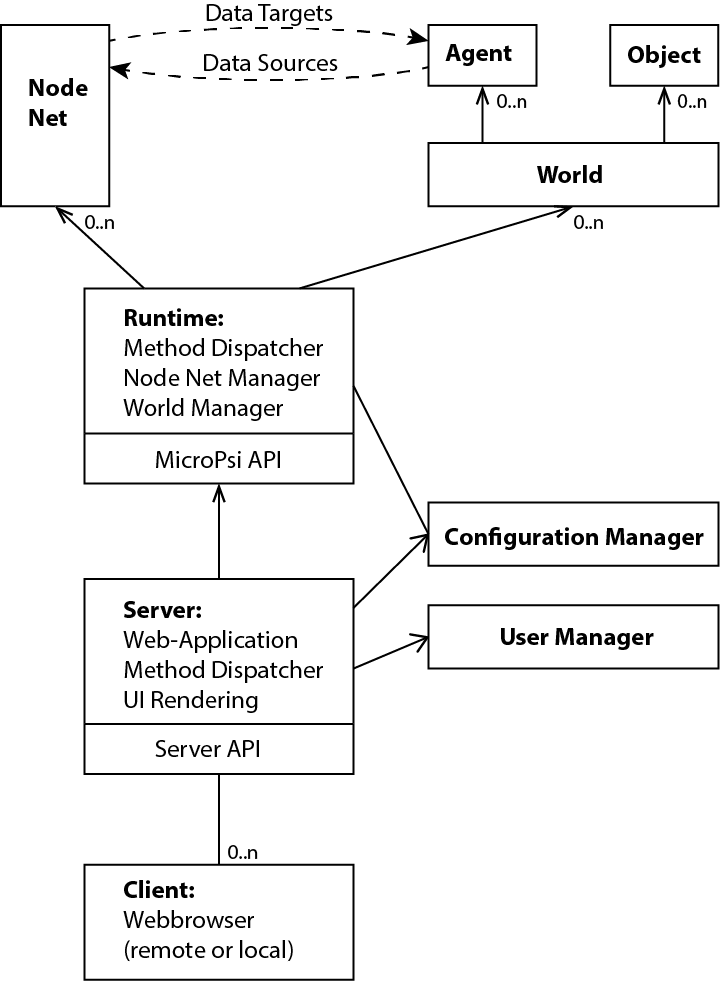
\includegraphics[width=5cm]{graphics/micropsi2_uml}

\subsection{Core}
... the core runs the heart of the simulation ...

\subsection{Server}
... the server provides the interface ...

\subsection{Simulation Environments}
... so far, there are an "Island" and an "Berlin" worlds ...

\section{A! Minecraft}
... a more complex simulation environment could be fun ...

... the story of Minecraft ...
... Minecrafts poularity (and demographics) ...

\subsection{What is Minecraft?}
... brief description of the basic mechanisms ...

\subsection{The Cient Server Protokoll}
... the language an external client needs to speak, to take place in a Minecraft world ...

\subsection{Suitability of Minecraft as a simulation environment}
... cheap licenses ...
... developer friendly community and game-studio ...
... sandbox game with many possibilieties but no pre-defined goals ...
... procedural semantic ...

\section{A! Minecraft and MicroPsi}
... a more complex simulation environment could be fun ...
\chapter{A! Approach / Minecraft as a Simulation Environment for MicroPsi 2}

\section{A! Overview / What has been there so far?}
... Minecraft Bots with simple as well as sophisticated AI ...
... MicroPsi 2 with Island and Berlin world ...

\section{A! Architecture / Building the interface in between Minecraft and the simulation environment}
... result: a Minecraft Bot that implements MicroPsi AI and is controlled and monitored via the MicroPsi webinterface ...
... the Webinterface holds its own visualization of the Agents worldview ...

\subsection{A Minecraft Bot}

\subsubsection{Protocol Implementation}

\subsubsection{Control Structures}

\subsubsection{Previous own implementations with TwistedBot}

\subsubsection{other popular Bot projects and game modifications}

\subsubsection{Spockbot von Nickelpro}

\section{Implementation}
% TODO je nach Größe des Kapitels, das hier vielleicht eine Ebene höher ziehen (versuche dich hier erstmal nur auf die fertige Lösung zu konzentrieren und warum du dich dafür entschieden hast. Es ist nicht interessant, was du sonst alles ausprobiert hast, außer dass du konkret angibst, warum du dich für die jetztige Implementierung im Vergleich zu anderen entschieden hast)

\section{Case Study}

\chapter{Conclusion}
%Analyse und Zusammenfassung / Auswertung der Ergebnisse / Diskussion der Ergebnisse und weitere Erkenntnisse / Limitationen und Ausblick

\section{What's next}
... what has been learned ...
... what can be done with the new environment ...
... what can be improved? ...
... what other simulation environments could be of interest? ...

% include more chapters

% optional
\begin{appendices}
	\chapter{Auszug aus dem Buch}
	Beispielhaft wird hier gezeigt, wie Block-Zitate eingeführt werden können. Hier der Beginn des Buchs "`Per Anhalter durch die Galaxis"' von Douglas Adams~\cite{adams1998anhalter_inbook}:
	
	\begin{quote}
	"`Das Haus stand auf einer kleinen Anhöhe genau am Rand des Ortes. Es stand alleine da und überblickte das weite Ackerland im Westen. Absolut kein bemerkenswertes Haus - es war ungefährt dreißig Jahre alt, plump, viereckig, aus Ziegelsteinen erbaut und hatte vier Fenster an der Vorderseite, der es nach Größe und Proportion mehr oder weniger mißlang, das Auge zu erfreuen."'
	\end{quote}
	
	\chapter{Implementierungen}
	Beispielhaft wird hier gezeigt, wie Code-Beispiele in den Text eingefügt werden können. Die Pseudocode-Umgebung wird von \emph{macros.tex} bereitgestellt und kann dort entsprechend angepasst werden.
			\begin{figure}[ht]
			\centering
			\begin{minipage}{11cm}
				\begin{pseudocode}
public static Object answeringMachine() {
	Thread.sleep(1000);
	return 42;
}
				\end{pseudocode}
				\caption{Implementierung einer Maschine zur Beantwortung der Fragen aller Fragen.}
				\label{IMG_PID}
			\end{minipage}
		\end{figure}
	
\end{appendices}

\backmatter % Do not move this command!

% optional
\phantomsection
\addcontentsline{toc}{chapter}{Abbildungsverzeichnis} % change according to language (adds the list of figures to the table of contents)
\listoffigures

% optional
\listoftables
\phantomsection
\addcontentsline{toc}{chapter}{Tabellenverzeichnis} % change according to language (adds the list of tables to the table of contents)

% change according to language
\chapter{Inhalt der beigelegten CD}
Die beigelegte CD enthält folgenden Inhalt:
\begin{itemize}
	\item diese Masterarbeit in PDF Format,
	\item Videos mit Interview von Fans,
	\item den Source-Code der Implementierung einer Maschine zur Beantwortung der Fragen aller Fragen. Der Source-Code ist im Ordner \emph{src} zu finden.
\end{itemize}
%%%%%%%%%%%%%%%%%%%%%%%%%%%%%%%%%%%%%
%%%%%%%%%%%%%%%%%%%%%%%%%%%%%%%%%%%%%

\cleardoublepage
\phantomsection
\addcontentsline{toc}{chapter}{Literaturverzeichnis} % change according to language (adds the bibliography to the table of contents)
\bibliographystyle{alphadin} % select this for a German thesis
%\bibliographystyle{alpha} % select this for an English thesis
\bibliography{thesis}


\end{document}